\documentclass[manuscript,screen,review]{acmart}

\usepackage{graphicx}
\graphicspath{ {./graphs/} }

\AtBeginDocument{%
  \providecommand\BibTeX{{%
    \normalfontB\kern-0.5em{\scshape i\kern-0.25em b}\kern-0.8em\TeX}}}

\setcopyright{acmcopyright}
\copyrightyear{2018}
\acmYear{2018}
\acmDOI{XXXXXXX.XXXXXXX}

\begin{document}

\title{Effectiveness Of Auditory Stressors In Military Training Environment}

\author{Laura S. Cook}
\email{cookls@colostate.edu}
\affiliation{%
  \institution{Colorado State University}
  \streetaddress{900 Oval Drive}
  \city{Fort Collins}
  \state{Coloradoio}
  \country{USA}
  \postcode{80523}
}
\author{Joshua J. Staut}
\email{jstaut53@colostate.edu}
\affiliation{%
  \institution{Colorado State University}
  \streetaddress{900 Oval Drive}
  \city{Fort Collins}
  \state{OhColoradoio}
  \country{USA}
  \postcode{80523}
}


\begin{abstract}
  Military training environments play a crucial role in preparing soldiers for protecting 
  the homeland. These environments are designed to train and equip individuals with the 
  proper skills and understanding to complete missions, execute orders, and safely return home. 
  This study was designed to better understand the effectiveness of auditory stressors in a training 
  environment in Air Force Reserve Officer Training Corps marching education. The study utilized 
  Virtual Reality (VR) technology to study the utilization of virtual environments to train and 
  educate college students on marching procedures. The research conducted will directly benefit 
  the format of training resources utilized at Detachment 090 at Colorado State University. This 
  research has the potential to help detachments across the United States better utilize 
  resources and train more effectively with schools that are spread out over the state they 
  reside in.  

The methodology for this experiment included participants that were cadets and civilians 
undergoing a VR experiment that included a teaching and testing phase. They indicated their 
confidence in performing marching movements both before and after the experiment to test whether 
their knowledge increased. The data analysis revealed that participants not exposed to auditory 
stressors outperformed from a correct move standpoint and in their confidence after the 
experiment. The experiment showed great promise in utilizing virtual environments for educational 
purposes and little support for using auditory stressors for improved performance.  

Overall, the analysis indicated that current practices of utilizing auditory stressors for increased 
performance in marching environments may be unnecessary. These findings support the idea that virtual 
or remote environments would be useful for those cadets that are separated by great distances from 
their host university. There also was an indication of broader use of VR technologies being applicable 
to training at the cadet and military levels. These insights provide a framework for reworking and 
optimizing training across the nation to better prepare cadets to enter active duty.  
\end{abstract}

\begin{CCSXML}
<ccs2012>
 <concept>
  <concept_id>10010520.10010553.10010562</concept_id>
  <concept_desc>Computer systems organization~Embedded systems</concept_desc>
  <concept_significance>500</concept_significance>
 </concept>
 <concept>
  <concept_id>10010520.10010575.10010755</concept_id>
  <concept_desc>Computer systems organization~Effectiveness</concept_desc>
  <concept_significance>300</concept_significance>
 </concept>
 <concept>
  <concept_id>10010520.10010553.10010554</concept_id>
  <concept_desc>Computer systems organization~Online Training</concept_desc>
  <concept_significance>100</concept_significance>
 </concept>
 <concept>
  <concept_id>10003033.10003083.10003095</concept_id>
  <concept_desc>Military~Leadership</concept_desc>
  <concept_significance>100</concept_significance>
 </concept>
</ccs2012>
\end{CCSXML}

\ccsdesc[500]{Computer systems organization~Embedded systems}
\ccsdesc[300]{Computer systems organization~Effectiveness}
\ccsdesc{Computer systems organization~Online Training}
\ccsdesc[100]{Military~Leadership}

\keywords{Auditory Stress, Military Training, Effectiveness, Training}

\received{29 March 2024}
\received[revised]{29 March 2024}
\received[accepted]{6 May 2024}

\maketitle

\section{Introduction}
Military training environments have historically served to standardize, equip, and 
prepare fighting forces in the United States of America. In practice, it is 
important to provide well-equipped individuals in all branches of service, 
including the United States Air Force. At Colorado State University individuals 
training to earn a commission as an officer in the United States Air Force attend 
Detachment 090. Cadets are trained in various settings, but the most emphasized is 
in a high-stress environment with auditory stressors. In these environments cadets 
are tested on their ability to perform under pressure in knowledge recall, marching 
practices, and personal bearing. At Detachment 90 there are multiple universities 
that are represented. One of these universities is over an hour drive from Colorado 
State University. Having an in-person training environment is not always possible for 
the individuals that attend the University of Northern Colorado. This study was 
designed to decide if auditory stressors are crucial to proper military training or 
if there is a potential for change in the design of curriculum at the Detachment.  

The study aimed to test the effectiveness of auditory stressors in an online military 
learning environment. This will be beneficial for remote training practices in our 
Detachment and could be applicable to other Detachments across the nation that serve 
multiple schools in spread out communities. Conducting this research gave us a better 
perspective of the effectiveness of our current training practices and provided insights 
into areas of improvement. This research helped deduce whether online training is a 
proper substitute for in person training at the Air Force Reserve Officer Training Corps 
level and the role of auditory stressors in both virtual and in person environments.   

\section{Related Works}
In other works, stressors have been shown in a virtual environment to simulate visual stressors
 and environments. For the purposes of our research, we are more interested in how loud noise 
 and pressure effects the individual and their performance since this is directly applicable 
 to the training practices used in person at Detachment 90. The results of this study could 
 help create a virtual training environment in the future or allow for a new perspective on in 
 person training environments in general. 

\subsection{Stress in Education}
In other works, stressors have been researched in an educational setting. We began our 
research by trying to understand the effects of stress on performance and in relation 
to retention and task completion. In the article “Critical brain circuits at the 
intersection between stress and learning”, the authors researched the psychological 
effects of stress on learning and retention. The study found that in many instances 
“stressful experience alters our ability to acquire or remember new information\ldots” 
[2]. These findings support the idea that stress and intensity may not be beneficial 
for academic environments overall. The article “Learning under stress: how does it work?”
 also looked at the effects of stress on learning, but through the lens of hormones 
 specifically. The study found that specifically if a stressor is presented during 
 learning and recall in the same way that there is a positive correlation between stress 
 and memory [9]. However, these conditions must be replicated in the same space and time 
 to produce a positive response [9]. Since our training environment is not consistent in 
 these conditions, the introduction of stressors may not be beneficial to our mission. 
 Another source suggested that stress can be useful in some situations but can depend 
 heavily on the novelty of the decision being made [15]. In relation to auditory stressors 
 directly, a final article took a deep dive into the auditory cortex and how it is not 
 just a sensor but can be linked to memory [18]. 

\subsection{Reseacrh Forming}
As we continued forming our research, we found that VR was the most effective educational 
platform for 3D learning [7]. In looking at other research we identified some areas of 
interest such as engagement, VR learning, and scalability [1]. We considered possible 
risk factors for our project and found constraints such as cybersickness and willingness 
to complete the project [12]. To combat these issues, we discovered the ability of 
individuals to be open and willing to change via the ABOS scale [6]. This gave us a 
unique look at different scales that could be used to gauge how willing future participants 
in this program might be to learn in this environment [6]. By developing this virtual 
environment, we needed to understand the importance of starting with VR as a medium. We 
found that it was beneficial to start a student's education of marching practices in 
a VR environment instead of teaching something one way and then changing later [3]. 
The article promoted the idea of virtual environment as a teaching tool used in 
educational settings [3]. Another source studied cognitive behavior and reaction 
time of 57 personnel undergoing an 18-week training to see how stressors commonly 
found in military environment affected factors such as visual object tests [16]. 
In these tests the personnel were given quizzes after being put under stressors [16]. 
This is an example we followed to conduct our research.   

\subsection{Stress in military scenario}
We decided to take a deeper dive into other research on stress as it relates to military 
scenarios which directly related to our research. Studies related to stress in military 
training environments vary from basic everyday stressors that impact forces to deploy 
specific stressors that are more intense than what is being researched for our purpose [4]. 
In some cases, virtual environments were implemented to simulate stressful environments 
such as deployment [4]. These scenarios were meant to produce a learning environment in 
which individuals can train responses and stay calm under extreme pressures [4]. Our 
research aimed to do this in the context of marching education but not live fire or 
anything of extreme nature. The report “Stress Training and the New Military Environment” 
looked at stress in military training environments and how they have evolved. The research 
conducted found that many individuals found high intensity training they endured to be 
necessary to handle the stress they were put under in combat situations [8]. However, 
many cadets that commission through the ROTC programs will not need such intense training 
for their day-to-day jobs. In fact, most special careers that demand this type of stress-based 
training will provide specific training before any kind of deployment or job-related incident.  

\subsection{Stress Training in a Military Environment}
Studies related to stress in military training environments vary from basic everyday stressors that 
impact forces to deploy specific stressors that are more intense than what is being researched for 
our purposes. In a paper titled “Selection of Key Stressors to Develop Virtual for Practicing Stress 
Management Skills with Military Personnel Prior to Deployment” virtual environments were implemented 
to simulate stressful environments. This source introduces virtual environments to familiarize service 
members with stressors in a deployed environment. These can include deceased individuals, someone being 
injured in front of them, and returned fire. These scenarios are meant to produce a learning environment 
in which individuals can train responses and stay calm under extreme pressures. Additional elements in 
this study include trying to decrease stress and provide a safe place to desensitize military members 
to graphic incidents to decrease PTSD response on return. This study was used for both deployments in 
combat and peacekeeping missions as both environments can put military personnel in situations that could 
lead to traumatic experiences.  

Some sources found that stress in military training had positive effects on results later in service. 
A source found that utilization of stress management techniques on screen in VR environments decreased 
stress levels and increased performance [5]. In a study on marching and marksmanship accuracy a 
10-20\% increase in marksmanship was indicated when completing rucks 
and marching exercises consistently [17]. Overall, it was seen that stress in training could be 
useful if implemented correctly. This led us to further question the ability for auditory stressors 
to positively impact marching performance in training versus live practice.  

\subsection{Military VR application}
The application of VR technology in a military setting is diverse and paints a picture of immense 
innovation moving forwards. One source gave an overview of applications to include military 
training in otherwise dangerous conditions and how military members felt more prepared to handle 
live fire or non-routine conditions as a result [19]. Another article detailed simulator capabilities 
dating back to the 1950s and specifically discussed how night flying training was previously incredibly 
risky, and this mitigated a lot of the possible complications [10]. In further research an overview 
of applications of VR to help with PTSD and cognitive repair following combat was proven successful 
[14]. From basic field training to weapons manufacturing education, there is a breadth of possibilities 
for VR environments to change the landscape of military education and reform [11].  

For the purposes of our research, we were more interested in how auditory stressors effect an individual 
and their performance as it directly applicable to the training practices used in person at Detachment 
090. However, other sources looked at the application of tailoring virtual environments to specific job 
training for military purposes [20]. This provided a broader understanding of tools that could be used 
for ensuring military training is used for something such as tactical field training. Although not directly 
tied to military research, another article discussed land geography accuracy in a VR environment, and 
this could be useful for land navigation which we do at Detachment 090 [13]. These articles helped us 
understand that our environment could be manipulated and altered to serve greater purposes in the future.   


\section{Methodology}
\subsection{Surveys}
Each participant began by answering a series of questions to include: How stressed do you feel on a scale 
of 1-10? How confident are you in your ability to perform a Right Facing movement on a scale of 1-10? How 
confident are you in your ability to perform a Left Facing movement on a scale of 1-10? How confident are 
you in your ability to perform a About Facing movement on a scale of 1-10? How confident are you in your 
ability to follow the command Present Arms on a scale of 1-10? How confident are you in your ability to 
follow the command Order Arms on a scale of 1-10? 

\subsection{Outline}
Each participant then was led through an instructional period where they were taught how to do each 
movement utilizing the Virtual Reality system. During this time a video was shown to the participant 
for each movement in the sequence. Each video went over the movement being performed three times. 
After being shown the movements, the participants were encouraged to practice the movements with the 
video. At the end of the instructional period, they entered a testing period. The participants were 
placed in two groups randomly, one with auditory stressors and background noise and one with only the 
commands being presented. The testing period went through each movement two or three times and recorded 
how many movements were completed correctly and how many times. The results of whether the movement was 
done correctly was done by the testers. Each participant got a 1 or 0 if it was correct and this was 
recorded and graphed. The criteria used for testing were timeliness of move, whether the move was in 
cadence, and accuracy of move, if the move was preformed correctly.  

\subsection{Application}
This coding was all done through Unity, a VR game development software. This was done to track movements 
to get an accurate and real-time reading of movements as the test was conducted. Through Unity we were 
able to get animated hands for the present/order arms movements and flawlessly play instructions through 
a made video. The Unity project was built and ran off a PC and through a quest Airlink was set up through 
an Oculus Rift 2. There were two major set up pieces for each participant. First, the PC was connected to 
a large monitor to watch the participants in real time as they completed the experiment. This was done so 
manual data tracking could be achieved. Second, the participants connected to the VR and made sure everything 
was set up before beginning the experiment.  

\subsection{Final Survey}
Following the instructional and testing period the participants answered the same questions as before. 
Their answers were recorded and compared to their initial responses. This was to gain some knowledge on 
how effective the participant felt in their ability before the training and after. This was to get a 
subjective view into the study of the auditory stressor's effectiveness

% \subsection{Begining Survey}
% Each participant began by answering a series of questions to include: How stressed do you feel on a scale of 1-10? 
% How confident are you in your ability to perform a Right Facing movement on a scale of 1-10? How confident are you 
% in your ability to perform a Left Facing movement on a scale of 1-10? How confident are you in your ability to perform 
% a About Facing movement on a scale of 1-10? How confident are you in your ability to follow the command Present Arms on 
% a scale of 1-10? How confident are you in your ability to follow the command Order Arms on a scale of 1-10? This was 
% done to gain a background on any participants. We can use this survey to compare both participants with knowledge of 
% military marching and those without. This way we helped eliminate any outside factors for the data collected. We preformed 
% the test on participants who had previous training and those with no experience at all. 

% \subsection{Instructional Period}
% Each participant then was led through an instructional period where they were taught how to do each movement utilizing the 
% Virtual Reality system. During this time a video was shown to the participant for each movement in the sequence. Each video 
% lasted two minutes with time to practice each movement. At the end of the ten-minute instructional period, they entered a 
% testing period. The participants were placed in two groups randomly, one with auditory stressors and background noise and 
% one with only the commands being presented. The testing period went through each movement three times and recorded how many 
% movements were completed correctly and how many times. The automated checkpoint system recorded this and whether auditory 
% stressors were utilized.

% \subsection{Testing Period}
% After the instructions the participants were put through the testing period. While in the VR Headset, a list of commands 
% was given out as seen in the instructional period. The group in the non-stressor environment were just be given the commands. 
% The group in the auditory stress environment were given both the commands as well as background stressors commonly found in 
% a training environment. These included yelling, loud noises from vehicles, and noises from firearms. The code implementation 
% used measured the movements of the participants. The participants were graded on a scale of doing the movements in time and the 
% accuracy of the movement preformed. The headset used had hand controls that will be the main source for this information. The 
% time was measured based on a standard cadence coded into the program. The participants were expected to match this cadence. 
% The measurement for time was the difference between the standard cadence and the performed cadence. The measure of accuracy 
% also heavily relied on the hand controls and the direction moved when performed. For example, did the right hand move when 
% “present” was called or did the user turn left when “left face” is called. The data was coded to record these data points 
% based on every command, each called twice.  This data was then graphed and compared from group to group. \par
% The stress-free instructional period was a simple video played through the headset, both demonstrating the movements 
% and getting the user used to the headset. The experiment relied heavily on subjects watching a video of marching procedure 
% and using this knowledge in an immediate test phase. The independent variable in this experiment was be added auditory 
% stressor while measuring the dependent variables of both time and accuracy. 

% \subsection{Follow-Up Survey}
% Following the instructional and testing period the participants answered the same questions as before. Their answers were 
% recorded and compared to their initial responses as well as their test data. This was done to gauge how participants 
% believed they performed. A huge part of military training is believing you can accomplish goals and objectives required of 
% you. The follow-up survey allowed us to get data on how auditory stress played a role in this part of training. One of the 
% main arguments against using auditory stressors in a training environment is it makes military personnel unwilling to 
% learn or grow. While this is not the focus of the experiment, it was vital data that was looked at. It gives an insight 
% into the mind behind the training to help further understand how military training can be improved.  

\section{Results}
As we did the experiment, we were testing mainly to find if the auditory stressor we used was effective in our 
VR training simulation. As we collected our data some interesting patterns came out of it. Below is a graph of data: 

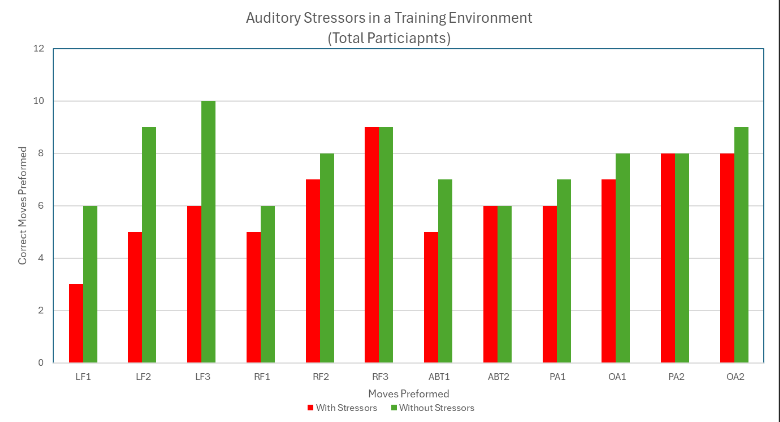
\includegraphics[scale=0.8]{MainGraph}

For almost every movement performed, the participants without the stressor in their test performed better than the 
participants with the stressor. We see that on average, all participants got better at the movement the more they 
performed it. This is a very common trend to see among experiments designed like ours. We had them performing 
three of the same movements, in some cases, and each of these three has an upward trend in the accurate completion 
rate. Again, however, those without the stressor had a significantly higher trend in almost every category. While 
some movements were relatively close, some (like left face) had almost a 50\% increase 
in accurate moves performed. This was an interesting piece of the data that was found, since as ROTC cadets we have 
been trained in a stressful environment for most of our careers.  

On average, those without the stressor had 7.75 people perform that move correctly with a total accuracy average of 
9.3 moves per person. This group had a standard deviation of 1.35 across the board. This showed that each participant 
had relatively equal experience and performed well on the testing portion of the experiment. The non-stressor group 
had a total of accurate moves performed of 93 moves. On the opposite side, those with the stressor had a lower average 
per move with only 6.3 people performing each move correctly, and a total accuracy average of 7.5 moves performed 
correctly per person. The stressor group had a standard deviation of 1.65 showing a more varied testing experience 
than those in the non-stressor group. This group had 75 total accurate moves performed. With an almost 30\% 
increase in accurate moves, this data heavily suggests that those in the non-stressor group were much more confident 
in those moves and had an overall better understanding of the objectives asked of them.  

One major bias we had in our data was also would we used as participants. Many of our testers were already in ROTC 
and have expereince with the moves we were looking to teach. This was one bias we were aware of going into the 
experiment and made sure to track to account for it. Below is a table graphing the difference between our non-ROTC 
testers and ROTC cadets.

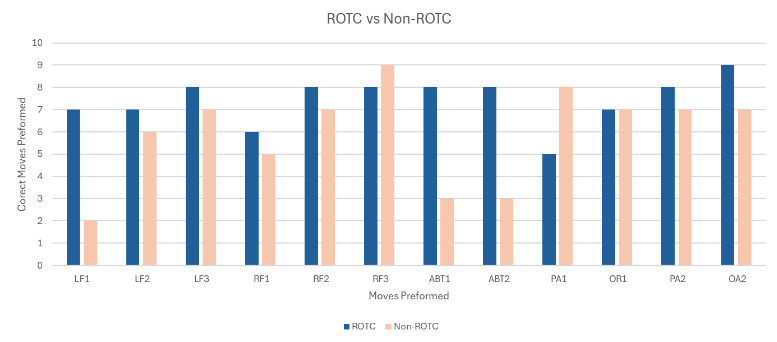
\includegraphics[scale=0.8]{ROTCGraph}

This was data we felt necessary to track as it played a major role in the outcome of our data. We even split the 
ROTC cadets into the stressor and non-stressor groups to try and mitigate the bias in our overall data. This data 
is about what we expected with the ROTC cadets having a significant accuracy average over the participants who had 
never seen these moves before. The performance for the ROTC cadets remained relatively level, with slight increases 
after reputation of moves. The non-ROTC group shows a rise in accuracy through this reptation that was seen in 
the first graph. The ROTC group had 89 total moves performed correctly compared to the other group with 73.   

Some of the reasons for this data may have been not only because the cadets had seen these moves before, but 
also because cadets are used to high pressure and stressful environments. As stated before, we are currently 
trained in these high-stress environments so every participant who is used to this had a clear advantage in the 
experiment. Though, by tracking this data, we learned something else about auditory stressors. The stressors 
did not have a significant role to play in training the ROTC cadets. It had a clear role in the civilians in 
the performance and overall accuracy, but not in the cadets themselves. This was fascinating to find, and it 
points to the conclusion that there is not a significant difference in training on the military front. Couple 
this with the data found in the overall research, and it led us to believe that it may be more beneficial to 
train military personnel without the use of auditory stressors.

\section{Discussion(Limitations)}
As the project unfolded, we ran into multiple limitations and standstills. We had originally planned to code 
the project in unity and create an automated game to record the movements of the participant. We found that 
this was incredibly challenging and due to our limited resources, we were unable to complete this on our 
personal computers. May weeks were spent trying to get the automated movement tracking working. However, 
this was the first time either of us had ever coded in C\# and used a software like Unity. 
The experiment itself came out clean and ready to use, however, the main problem was the movement tracking and more 
importantly the exportation of this data. Any data collected from the game was unreadable or incredibly 
hard to use. This led to us having to manually collect the data based off personal understanding of the 
drill movements. It would have been much nicer and an overall cleaner project if we could have gotten 
this tracking system working. This would have allowed us to not only track the accuracy of each movement, 
but also the exact timing of the movements to track the cadence in which they were performed.  

In the project both XR requirements and animations were completed so the user could interact with the 
experiment as they performed it. This allowed for a much more realistic feeling when the testers were 
inside. They could still interact with the system and this piece of the experiment came out great. This 
allowed for accurate (though limited) data collection. This part of the project went very well and turned 
out to allow the user to interact with the system. 

\section{Conclusion and Future Work}
The problem we initially set out to answer ended up being very complex in nature as our research unfolded 
and we became more educated on teaching practices and stressors in general. A seemingly easy decision to 
choose a VR platform for our project was discovered to be both more beneficial to education and more 
difficult in application than we imagined. As we formulated our process and techniques, we discovered 
how beneficial the technology could be to additional applications for teaching within our Detachment. 
Through experimentation, we saw our results come to life and taught individuals with no prior marching 
experience the techniques we had spent ten years collectively learning and perfecting.  

We hope to present these findings to our leaders and decision makers in hopes that positive change 
could result in our education at Detachment 090. We believe that given our findings it is unnecessary 
to rely on auditory stressors in a training environment and a remote or virtual environment would be 
beneficial to supplement instruction time face to face. This would need to be further researched for 
applications such as warrior knowledge, land navigation, tactical exercises, and more. However, given 
our positive results and related works research, we believe that VR would be an excellent educational 
tool for multiple applications at Detachment 090 and beyond.\\ \\ \\ \\ \\ \\ \\

\section{References}
\begin{verbatim}
  [1] Akdere, M. (2021). Virtual Reality Technology for developing Intercultural Leadership Competence: 
      A research proposal. European Proceedings of Social and Behavioural Sciences. 
      https://doi.org/10.15405/epsbs.2021.02.17  

  [2] Bangasser, D. A., & Shors, T. J. (2010). Critical brain circuits at the intersection between 
      stress and learning. Neuroscience &amp; Biobehavioral Reviews, 34(8), 1223–1233. 
      https://doi.org/10.1016/j.neubiorev.2010.02.002  
  
  [3] Bossard, C., Kermarrec, G., Buche, C., & Tisseau, J. (2008). Transfer of learning in virtual 
      environments: A new challenge? Virtual Reality, 12(3), 151–161. 
      https://doi.org/10.1007/s10055-008-0093-y  
  
  [4] Bouchard, S., Baus, O., Bernier, F., & McCreary, D. R. (2010). Selection of key stressors to 
      develop virtual environments for practicing stress management skills with military personnel 
      prior to deployment. Cyberpsychology, Behavior, and Social Networking, 13(1), 83–94. 
      https://doi.org/10.1089/cyber.2009.0336  
  
  [5] Bouchard, S., Bernier, F., Boivin, É., Morin, B., & Robillard, G. (2012). Using biofeedback 
      while immersed in a stressful videogame increases the effectiveness of stress management 
      skills in soldiers. PLoS ONE, 7(4). 
      https://doi.org/10.1371/journal.pone.0036169  
  
  [6] Caligiuri, P. M., Jacobs, R. R., & Farr, J. L. (2000). The attitudinal and behavioral 
      openness scale: Scale Development and construct validation. International Journal of 
      Intercultural Relations, 24(1), 27–46. 
      https://doi.org/10.1016/s0147-1767(99)00021-8  
  
  [7] Chao, C., Wu, S., Yau, Y., Feng, W., & Tseng, F. (2017). Effects of three‐dimensional 
      virtual reality and traditional training methods on mental workload and training 
      performance. Human Factors and Ergonomics in Manufacturing &amp; 
      Service Industries, 27(4), 187–196. 
      https://doi.org/10.1002/hfm.20702  
  
  [8] Delahaij, R., & Soeters, J. M. (2007, October 17). Stress Training and the New Military 
      Environment. Defense Technical Information Center. 
      https://apps.dtic.mil/sti/citations/tr/ADA472722   
  
  [9] Joëls, M., Pu, Z., Wiegert, O., Oitzl, M. S., & Krugers, H. J. (2006). Learning under stress: 
      How does it work? Trends in Cognitive Sciences, 10(4), 152–158. 
      https://doi.org/10.1016/j.tics.2006.02.002  
  
  [10] Lele, A. (2011). Virtual reality and its military utility. Journal of Ambient Intelligence 
       and Humanized Computing, 4(1), 17–26. 
       https://doi.org/10.1007/s12652-011-0052-4  
  
  [11] Liu, X., Zhang, J., Hou, G., & Wang, Z. (2018). Virtual reality and its application in 
       military. IOP Conference Series: Earth and Environmental Science, 170, 032155. 
       https://doi.org/10.1088/1755-1315/170/3/032155  
  
  [12] MICHALSKA, A., KONOPACKI, M. M., & RODZIK, D. (2024). Study of adverse factors during 
       training with virtual reality simulator. Inżynieria Bezpieczeństwa Obiektów 
       Antropogenicznych, (1), 35–48. 
       https://doi.org/10.37105/iboa.205  
  
  [13] Putra, A. K., Al Khalidy, D., Handoyo, B., & Van Thang, H. (2023). Construction of 
       immersive experiences: Development of virtual reality technology to facilitate physical 
       geography learning. International Journal of Emerging Technologies 
       in Learning (iJET), 18(19), 47–60. 
       https://doi.org/10.3991/ijet.v18i19.40859  
  
  [14] Rizzo, A. (2012). Virtual reality goes to war: Recent advances in military behavioral 
       healthcare. PsycEXTRA Dataset. 
       https://doi.org/10.1037/e533652013-136  
  
  [15] Sarmiento, L. F., Lopes da Cunha, P., Tabares, S., Tafet, G., & Gouveia Jr, A. (2024). 
       Decision-making under stress: A psychological and neurobiological integrative model. 
       Brain, Behavior, &amp; Immunity - Health, 38, 100766. 
       https://doi.org/10.1016/j.bbih.2024.100766  
  
  [16] Tait, J. L., Aisbett, B., Corrigan, S. L., Drain, J. R., & Main, L. C. (2022). Recovery 
       of cognitive performance following multi-stressor military training. Human Factors: 
       The Journal of the Human Factors and Ergonomics Society, 66(2), 389–403. 
       https://doi.org/10.1177/00187208221086686  
  
  [17] Tenan, M. S., LaFiandra, M. E., & Ortega, S. V. (2016). The effect of soldier marching, 
       rucksack load, and heart rate on Marksmanship. Human Factors: The Journal of the Human 
       Factors and Ergonomics Society, 59(2), 259–267. 
       https://doi.org/10.1177/0018720816671604  
  
  [18] Weinberger, N. M. (2015). New Perspectives on the auditory cortex. The Human Auditory 
       System - Fundamental Organization and Clinical Disorders, 117–147. 
       https://doi.org/10.1016/b978-0-444-62630-1.00007-x  
  
  [19] Xie, B., Liu, H., Alghofaili, R., Zhang, Y., Jiang, Y., Lobo, F. D., Li, C., Li, W., 
       Huang, H., Akdere, M., Mousas, C., & Yu, L.-F. (2021). A review on Virtual reality 
       skill training applications. Frontiers in Virtual Reality, 2. 
       https://doi.org/10.3389/frvir.2021.645153  
  
  [20] Zook, A., Lee-Urban, S., Riedl, M. O., Holden, H. K., Sottilare, R. A., & Brawner, K. W. 
       (2012). Automated scenario generation. Proceedings of the International Conference on the 
       Foundations of Digital Games. 
       https://doi.org/10.1145/2282338.2282371 
\end{verbatim}

\end{document}
\endinput

